\begin{enumerate}[label=\arabic*.,ref=\thesection.\theenumi]
\numberwithin{equation}{enumi}
\item Construct a Transmitter circuit.
\\
\solution:
\begin{figure}[H]
\centering
  \begin{figure}[H]
\begin{circuitikz} [scale=.73,font=\footnotesize]

%\draw (5,5) -- (6.5,5) to[R=$R_4:47k\Omega$, label=$\mathrm{R_4}$, left] (6.5,2);

\draw (0,0) node[circ] {} to[C=$C_1$] node[pos=0.07,below left=1.5ex]{\SI{0.1}{\mu F}} ++(3.7,0) node[npn, anchor=B] (Q1) {$Q_1$};
\draw(4.85,-0.5)--(4.85,-4);
%\draw (0,0) -- (0,5) toR=$R_3 47k\Omega$;
\draw (0,0)--(0,5) to[R=$R_3$]  node[pos=0.05,below left=1.5ex]{\SI{47}{k\Omega}}(5,5);
\draw (3,0)--(3,2) to[R=$R_1$]  node[pos=0.05,below left=1.5ex]{\SI{1}{M\Omega}}(4.85,2)--(4.85,.5);
\draw (4.8,2)--(5,2) to[C=$C_2$]node[pos=1.8,below left=1.2ex]{\SI{0.1}{\mu F}} (6.5,2);
%\draw(4.85,2)--(4.85,2.5) toR=$R_2:10k\Omega$;
\draw (4.85,2)--(4.85,2.5) to[R=$R_2$]  node[pos=0.15,below left=1ex]{\SI{10}{k\Omega}}(4.85,5);
\draw (5,5) -- (6.5,5) to[ R]node[pos=-1.5,above left]{$R_4$} node[pos=-0.8,above left=1ex]{\SI{47}{k\Omega}} (6.5,2);
%\draw (5,5) -- (6.5,5) to[R=$R_4$]node[pos=0.1,above right=1ex]{\SI{47}{k\Omega}}(6.5,2);
\draw (6.5,2)--(6.5,-2) to[C=$C_3$] node[pos=-0.01,above left=1.5ex]{\SI{1}{ nF}} (6.5,-4);
\draw (0,0)--(0,-2) to [mic]node[pos=0.08,above right=2ex]{mic}(0,-4);
\draw(6.5,5)--(9,5);
\draw (9,5)--(9,4.5);

\draw(9,4.5)--(7.5,4.5)to[C=$C_6$]node[pos=0.01,above right=1.5ex]{\SI{33}{pF}} (7.5,2.5);
 %\draw(9,4.5)--(7.75,4.5)to[C]node[pos=-1.2,above left]{$C_6$} node[pos=-0.5,above left=1ex]{\SI{33}{pF}} (7.75,2.5);
\draw(9,4.5)to[C=$C_5$]node[pos=0.01,above right=1.5ex]{\SI{33}{pF}} (9,2.5);
\draw(7.5,4.5)--(10.5,4.5)to[L=$L_1$] node[pos=1.2,above right=2.5ex]{\SI{1}{\mu H}} (10.5,2.5);
\draw (7.5,2.5)--(10.5,2.5);
\draw(9,2.5)to[C=$C_4$] node[pos=0.01,below right=1.5ex]{\SI{10}{pF}} (9,-1.5);
\draw(9,-1.5)--(7.75,-1.5);
\draw(6.5,0)--(6.6,0);
\draw(0,0) ++(6.6,0) node[npn, anchor=B] (Q2){$Q_2$};
\draw(7.74,.5)--(7.74,1.5)--(9,1.5);
\draw(7.74,-0.5)--(7.74,-1.5);
\draw(7.74,-1.5)to[R=$R_5\ 470\Omega$] (7.74,-4);
\draw(9,1.5)--(9.75,1.5)to[C=$C_7$]node[pos=0.01,below right=1.5ex]{\SI{10}{pF}}  (10,1.5);
\draw(10,1.5)--(11,1.5);
\draw(11,1.5)--(11,2.5) node[antenna] {antenna};
\draw(9,5)--(12.5,5)to[C=$C_8$] node[pos=0.05,below left=1.5ex]{\SI{0.1}{\mu F}}(12.5,-4);
\draw(12.5,5)--(14.5,5);
\draw (14.5, -4) to [battery](14.5, 5);
\draw(0,-4)--(14.5,-4);
\end{circuitikz}
\label{fig:tx_cir}
\end{figure}

  \caption{FM Transmitter Circuit diagram}
  \label{ckt:circuit_2}
\end{figure}
\item List the components in the transmitter circuit diagram.\\
\solution \\
\begin{table}[!ht]
  \centering
  %%%%%%%%%%%%%%%%%%%%%%%%%%%%%%%%%%%%%%%%%%%%%%%%%%%%%%%%%%%%%%%%%%%%%%
%%                                                                  %%
%%  This is the header of a LaTeX2e file exported from Gnumeric.    %%
%%                                                                  %%
%%  This file can be compiled as it stands or included in another   %%
%%  LaTeX document. The table is based on the longtable package so  %%
%%  the longtable options (headers, footers...) can be set in the   %%
%%  preamble section below (see PRAMBLE).                           %%
%%                                                                  %%
%%  To include the file in another, the following two lines must be %%
%%  in the including file:                                          %%
%%        \def\inputGnumericTable{}                                 %%
%%  at the beginning of the file and:                               %%
%%        \input{name-of-this-file.tex}                             %%
%%  where the table is to be placed. Note also that the including   %%
%%  file must use the following packages for the table to be        %%
%%  rendered correctly:                                             %%
%%    \usepackage[latin1]{inputenc}                                 %%
%%    \usepackage{color}                                            %%
%%    \usepackage{array}                                            %%
%%    \usepackage{longtable}                                        %%
%%    \usepackage{calc}                                             %%
%%    \usepackage{multirow}                                         %%
%%    \usepackage{hhline}                                           %%
%%    \usepackage{ifthen}                                           %%
%%  optionally (for landscape tables embedded in another document): %%
%%    \usepackage{lscape}                                           %%
%%                                                                  %%
%%%%%%%%%%%%%%%%%%%%%%%%%%%%%%%%%%%%%%%%%%%%%%%%%%%%%%%%%%%%%%%%%%%%%%



%%  This section checks if we are begin input into another file or  %%
%%  the file will be compiled alone. First use a macro taken from   %%
%%  the TeXbook ex 7.7 (suggestion of Han-Wen Nienhuys).            %%
\def\ifundefined#1{\expandafter\ifx\csname#1\endcsname\relax}


%%  Check for the \def token for inputed files. If it is not        %%
%%  defined, the file will be processed as a standalone and the     %%
%%  preamble will be used.                                          %%
\ifundefined{inputGnumericTable}

%%  We must be able to close or not the document at the end.        %%
	\def\gnumericTableEnd{\end{document}}


%%%%%%%%%%%%%%%%%%%%%%%%%%%%%%%%%%%%%%%%%%%%%%%%%%%%%%%%%%%%%%%%%%%%%%
%%                                                                  %%
%%  This is the PREAMBLE. Change these values to get the right      %%
%%  paper size and other niceties.                                  %%
%%                                                                  %%
%%%%%%%%%%%%%%%%%%%%%%%%%%%%%%%%%%%%%%%%%%%%%%%%%%%%%%%%%%%%%%%%%%%%%%

	\documentclass[12pt%
			  %,landscape%
                    ]{report}
       \usepackage[latin1]{inputenc}
       \usepackage{fullpage}
       \usepackage{color}
       \usepackage{array}
       \usepackage{longtable}
       \usepackage{calc}
       \usepackage{multirow}
       \usepackage{hhline}
       \usepackage{ifthen}

	\begin{document}


%%  End of the preamble for the standalone. The next section is for %%
%%  documents which are included into other LaTeX2e files.          %%
\else

%%  We are not a stand alone document. For a regular table, we will %%
%%  have no preamble and only define the closing to mean nothing.   %%
    \def\gnumericTableEnd{}

%%  If we want landscape mode in an embedded document, comment out  %%
%%  the line above and uncomment the two below. The table will      %%
%%  begin on a new page and run in landscape mode.                  %%
%       \def\gnumericTableEnd{\end{landscape}}
%       \begin{landscape}


%%  End of the else clause for this file being \input.              %%
\fi

%%%%%%%%%%%%%%%%%%%%%%%%%%%%%%%%%%%%%%%%%%%%%%%%%%%%%%%%%%%%%%%%%%%%%%
%%                                                                  %%
%%  The rest is the gnumeric table, except for the closing          %%
%%  statement. Changes below will alter the table's appearance.     %%
%%                                                                  %%
%%%%%%%%%%%%%%%%%%%%%%%%%%%%%%%%%%%%%%%%%%%%%%%%%%%%%%%%%%%%%%%%%%%%%%

\providecommand{\gnumericmathit}[1]{#1} 
%%  Uncomment the next line if you would like your numbers to be in %%
%%  italics if they are italizised in the gnumeric table.           %%
%\renewcommand{\gnumericmathit}[1]{\mathit{#1}}
\providecommand{\gnumericPB}[1]%
{\let\gnumericTemp=\\#1\let\\=\gnumericTemp\hspace{0pt}}
 \ifundefined{gnumericTableWidthDefined}
        \newlength{\gnumericTableWidth}
        \newlength{\gnumericTableWidthComplete}
        \newlength{\gnumericMultiRowLength}
        \global\def\gnumericTableWidthDefined{}
 \fi
%% The following setting protects this code from babel shorthands.  %%
 \ifthenelse{\isundefined{\languageshorthands}}{}{\languageshorthands{english}}
%%  The default table format retains the relative column widths of  %%
%%  gnumeric. They can easily be changed to c, r or l. In that case %%
%%  you may want to comment out the next line and uncomment the one %%
%%  thereafter                                                      %%
\providecommand\gnumbox{\makebox[0pt]}
%%\providecommand\gnumbox[1][]{\makebox}

%% to adjust positions in multirow situations                       %%
\setlength{\bigstrutjot}{\jot}
\setlength{\extrarowheight}{\doublerulesep}

%%  The \setlongtables command keeps column widths the same across  %%
%%  pages. Simply comment out next line for varying column widths.  %%
\setlongtables

\setlength\gnumericTableWidth{%
	103pt+%
	85pt+%
	90pt+%
0pt}
\def\gumericNumCols{3}
\setlength\gnumericTableWidthComplete{\gnumericTableWidth+%
         \tabcolsep*\gumericNumCols*2+\arrayrulewidth*\gumericNumCols}
\ifthenelse{\lengthtest{\gnumericTableWidthComplete > \linewidth}}%
         {\def\gnumericScale{1*\ratio{\linewidth-%
                        \tabcolsep*\gumericNumCols*2-%
                        \arrayrulewidth*\gumericNumCols}%
{\gnumericTableWidth}}}%
{\def\gnumericScale{1}}

%%%%%%%%%%%%%%%%%%%%%%%%%%%%%%%%%%%%%%%%%%%%%%%%%%%%%%%%%%%%%%%%%%%%%%
%%                                                                  %%
%% The following are the widths of the various columns. We are      %%
%% defining them here because then they are easier to change.       %%
%% Depending on the cell formats we may use them more than once.    %%
%%                                                                  %%
%%%%%%%%%%%%%%%%%%%%%%%%%%%%%%%%%%%%%%%%%%%%%%%%%%%%%%%%%%%%%%%%%%%%%%

\ifthenelse{\isundefined{\gnumericColA}}{\newlength{\gnumericColA}}{}\settowidth{\gnumericColA}{\begin{tabular}{@{}p{103pt*\gnumericScale}@{}}x\end{tabular}}
\ifthenelse{\isundefined{\gnumericColB}}{\newlength{\gnumericColB}}{}\settowidth{\gnumericColB}{\begin{tabular}{@{}p{85pt*\gnumericScale}@{}}x\end{tabular}}
\ifthenelse{\isundefined{\gnumericColC}}{\newlength{\gnumericColC}}{}\settowidth{\gnumericColC}{\begin{tabular}{@{}p{90pt*\gnumericScale}@{}}x\end{tabular}}

\begin{longtable}[c]{%
	b{\gnumericColA}%
	b{\gnumericColB}%
	b{\gnumericColC}%
	}

%%%%%%%%%%%%%%%%%%%%%%%%%%%%%%%%%%%%%%%%%%%%%%%%%%%%%%%%%%%%%%%%%%%%%%
%%  The longtable options. (Caption, headers... see Goosens, p.124) %%
%	\caption{The Table Caption.}             \\	%
% \hline	% Across the top of the table.
%%  The rest of these options are table rows which are placed on    %%
%%  the first, last or every page. Use \multicolumn if you want.    %%

%%  Header for the first page.                                      %%
%	\multicolumn{3}{c}{The First Header} \\ \hline 
%	\multicolumn{1}{c}{colTag}	%Column 1
%	&\multicolumn{1}{c}{colTag}	%Column 2
%	&\multicolumn{1}{c}{colTag}	\\ \hline %Last column
%	\endfirsthead

%%  The running header definition.                                  %%
%	\hline
%	\multicolumn{3}{l}{\ldots\small\slshape continued} \\ \hline
%	\multicolumn{1}{c}{colTag}	%Column 1
%	&\multicolumn{1}{c}{colTag}	%Column 2
%	&\multicolumn{1}{c}{colTag}	\\ \hline %Last column
%	\endhead

%%  The running footer definition.                                  %%
%	\hline
%	\multicolumn{3}{r}{\small\slshape continued\ldots} \\
%	\endfoot

%%  The ending footer definition.                                   %%
%	\multicolumn{3}{c}{That's all folks} \\ \hline 
%	\endlastfoot
%%%%%%%%%%%%%%%%%%%%%%%%%%%%%%%%%%%%%%%%%%%%%%%%%%%%%%%%%%%%%%%%%%%%%%

\hhline{|-|-|-}
	 \multicolumn{1}{|p{\gnumericColA}|}%
	{\gnumericPB{\raggedright}\gnumbox[l]{\textbf{Component}}}
	&\multicolumn{1}{p{\gnumericColB}|}%
	{\gnumericPB{\raggedright}\gnumbox[l]{\textbf{Quantity}}}
	&\multicolumn{1}{p{\gnumericColC}|}%
	{\gnumericPB{\raggedright}\gnumbox[l]{\textbf{Value}}}
\\
\hhline{|---|}
	 \multicolumn{1}{|p{\gnumericColA}|}%
	{\gnumericPB{\raggedright}\gnumbox[l]{Transistor}}
	&\multicolumn{1}{p{\gnumericColB}|}%
	{\gnumericPB{\raggedleft}\gnumbox[r]{2}}
	&\multicolumn{1}{p{\gnumericColC}|}%
	{\gnumericPB{\raggedright}\gnumbox[l]{2N3904}}
\\
\hhline{|---|}
	 \multicolumn{1}{|p{\gnumericColA}|}%
	{\gnumericPB{\raggedright}\gnumbox[l]{Inductor}}
	&\multicolumn{1}{p{\gnumericColB}|}%
	{\gnumericPB{\raggedleft}\gnumbox[r]{1}}
	&\multicolumn{1}{p{\gnumericColC}|}%
	{\gnumericPB{\raggedright}\gnumbox[l]{1$\mu$H}}
\\
\hhline{|---|}
	 \multicolumn{1}{|p{\gnumericColA}|}%
	{\gnumericPB{\raggedright}\gnumbox[l]{Resistor}}
	&\multicolumn{1}{p{\gnumericColB}|}%
	{\gnumericPB{\raggedleft}\gnumbox[r]{1}}
	&\multicolumn{1}{p{\gnumericColC}|}%
	{\gnumericPB{\raggedleft}\gnumbox[r]{1M$\Omega$}}
\\
%\hhline{|---|}
	 \multicolumn{1}{|p{\gnumericColA}|}%
	{}
	&\multicolumn{1}{p{\gnumericColB}|}%
	{\gnumericPB{\raggedleft}\gnumbox[r]{1}}
	&\multicolumn{1}{p{\gnumericColC}|}%
	{\gnumericPB{\raggedleft}\gnumbox[r]{470$\Omega$}}
\\
%\hhline{|---|}
	 \multicolumn{1}{|p{\gnumericColA}|}%
	{}
	&\multicolumn{1}{p{\gnumericColB}|}%
	{\gnumericPB{\raggedleft}\gnumbox[r]{2}}
	&\multicolumn{1}{p{\gnumericColC}|}%
	{\gnumericPB{\raggedright}\gnumbox[l]{47k$\Omega$}}
\\
%\hhline{|---|}
	 \multicolumn{1}{|p{\gnumericColA}|}%
	{}
	&\multicolumn{1}{p{\gnumericColB}|}%
	{\gnumericPB{\raggedleft}\gnumbox[r]{1}}
	&\multicolumn{1}{p{\gnumericColC}|}%
	{\gnumericPB{\raggedright}\gnumbox[l]{10k$\Omega$}}
\\
\hhline{|---|}
	 \multicolumn{1}{|p{\gnumericColA}|}%
	{\gnumericPB{\raggedright}\gnumbox[l]{Capacitor}}
	&\multicolumn{1}{p{\gnumericColB}|}%
	{}
	&\multicolumn{1}{p{\gnumericColC}|}%
	{\gnumericPB{\raggedright}\gnumbox[l]{1nF}}
\\
%\hhline{|---|}
	 \multicolumn{1}{|p{\gnumericColA}|}%
	{}
	&\multicolumn{1}{p{\gnumericColB}|}%
	{\gnumericPB{\raggedleft}\gnumbox[r]{3}}
	&\multicolumn{1}{p{\gnumericColC}|}%
	{\gnumericPB{\raggedright}\gnumbox[l]{0.1$\mu$F}}
\\
%\hhline{|---|}
	 \multicolumn{1}{|p{\gnumericColA}|}%
	{}
	&\multicolumn{1}{p{\gnumericColB}|}%
	{\gnumericPB{\raggedleft}\gnumbox[r]{2}}
	&\multicolumn{1}{p{\gnumericColC}|}%
	{\gnumericPB{\raggedright}\gnumbox[l]{10pF}}
\\
%\hhline{|---|}
	 \multicolumn{1}{|p{\gnumericColA}|}%
	{}
	&\multicolumn{1}{p{\gnumericColB}|}%
	{\gnumericPB{\raggedleft}\gnumbox[r]{2}}
	&\multicolumn{1}{p{\gnumericColC}|}%
	{\gnumericPB{\raggedright}\gnumbox[l]{3.3pF}}
\\
\hhline{|---|}
	 \multicolumn{1}{|p{\gnumericColA}|}%
	{\gnumericPB{\raggedright}\gnumbox[l]{Antenna}}
	&\multicolumn{1}{p{\gnumericColB}|}%
	{\gnumericPB{\raggedleft}\gnumbox[r]{1}}
	&\multicolumn{1}{p{\gnumericColC}|}%
	{}
\\
\hhline{|---|}
	 \multicolumn{1}{|p{\gnumericColA}|}%
	{\gnumericPB{\raggedright}\gnumbox[l]{Condenser mic}}
	&\multicolumn{1}{p{\gnumericColB}|}%
	{\gnumericPB{\raggedleft}\gnumbox[r]{1}}
	&\multicolumn{1}{p{\gnumericColC}|}%
	{}
\\
\hhline{|-|-|-|}
\end{longtable}

\ifthenelse{\isundefined{\languageshorthands}}{}{\languageshorthands{\languagename}}
\gnumericTableEnd

  \caption{Transmitter components}
  \label{tab:tab_2}
\end{table}
\item The modulated signal is given by 
\begin{align}
	s(t) = \cos\brak{2\pi f_c t + \phi(t)}
\end{align}
where
\begin{align}
	\phi(t) = 2\pi k_f \int_{0}^{t}m(\tau)\,d\tau
	\label{4.2.2.2}
\end{align}
List the various parameters in a table.
\\
\solution
Parameters are in the table \tabref{tab:tab_1}
\vspace{10mm}
\begin{table}[!ht]
  \centering
  %%%%%%%%%%%%%%%%%%%%%%%%%%%%%%%%%%%%%%%%%%%%%%%%%%%%%%%%%%%%%%%%%%%%%%
%%                                                                  %%
%%  This is the header of a LaTeX2e file exported from Gnumeric.    %%
%%                                                                  %%
%%  This file can be compiled as it stands or included in another   %%
%%  LaTeX document. The table is based on the longtable package so  %%
%%  the longtable options (headers, footers...) can be set in the   %%
%%  preamble section below (see PRAMBLE).                           %%
%%                                                                  %%
%%  To include the file in another, the following two lines must be %%
%%  in the including file:                                          %%
%%        \def\inputGnumericTable{}                                 %%
%%  at the beginning of the file and:                               %%
%%        \input{name-of-this-file.tex}                             %%
%%  where the table is to be placed. Note also that the including   %%
%%  file must use the following packages for the table to be        %%
%%  rendered correctly:                                             %%
%%    \usepackage[latin1]{inputenc}                                 %%
%%    \usepackage{color}                                            %%
%%    \usepackage{array}                                            %%
%%    \usepackage{longtable}                                        %%
%%    \usepackage{calc}                                             %%
%%    \usepackage{multirow}                                         %%
%%    \usepackage{hhline}                                           %%
%%    \usepackage{ifthen}                                           %%
%%  optionally (for landscape tables embedded in another document): %%
%%    \usepackage{lscape}                                           %%
%%                                                                  %%
%%%%%%%%%%%%%%%%%%%%%%%%%%%%%%%%%%%%%%%%%%%%%%%%%%%%%%%%%%%%%%%%%%%%%%



%%  This section checks if we are begin input into another file or  %%
%%  the file will be compiled alone. First use a macro taken from   %%
%%  the TeXbook ex 7.7 (suggestion of Han-Wen Nienhuys).            %%
\def\ifundefined#1{\expandafter\ifx\csname#1\endcsname\relax}


%%  Check for the \def token for inputed files. If it is not        %%
%%  defined, the file will be processed as a standalone and the     %%
%%  preamble will be used.                                          %%
\ifundefined{inputGnumericTable}

%%  We must be able to close or not the document at the end.        %%
	\def\gnumericTableEnd{\end{document}}


%%%%%%%%%%%%%%%%%%%%%%%%%%%%%%%%%%%%%%%%%%%%%%%%%%%%%%%%%%%%%%%%%%%%%%
%%                                                                  %%
%%  This is the PREAMBLE. Change these values to get the right      %%
%%  paper size and other niceties.                                  %%
%%                                                                  %%
%%%%%%%%%%%%%%%%%%%%%%%%%%%%%%%%%%%%%%%%%%%%%%%%%%%%%%%%%%%%%%%%%%%%%%

	\documentclass[12pt%
			  %,landscape%
                    ]{report}
       \usepackage[latin1]{inputenc}
       \usepackage{fullpage}
       \usepackage{color}
       \usepackage{array}
       \usepackage{longtable}
       \usepackage{calc}
       \usepackage{multirow}
       \usepackage{hhline}
       \usepackage{ifthen}

	\begin{document}


%%  End of the preamble for the standalone. The next section is for %%
%%  documents which are included into other LaTeX2e files.          %%
\else

%%  We are not a stand alone document. For a regular table, we will %%
%%  have no preamble and only define the closing to mean nothing.   %%
    \def\gnumericTableEnd{}

%%  If we want landscape mode in an embedded document, comment out  %%
%%  the line above and uncomment the two below. The table will      %%
%%  begin on a new page and run in landscape mode.                  %%
%       \def\gnumericTableEnd{\end{landscape}}
%       \begin{landscape}


%%  End of the else clause for this file being \input.              %%
\fi

%%%%%%%%%%%%%%%%%%%%%%%%%%%%%%%%%%%%%%%%%%%%%%%%%%%%%%%%%%%%%%%%%%%%%%
%%                                                                  %%
%%  The rest is the gnumeric table, except for the closing          %%
%%  statement. Changes below will alter the table's appearance.     %%
%%                                                                  %%
%%%%%%%%%%%%%%%%%%%%%%%%%%%%%%%%%%%%%%%%%%%%%%%%%%%%%%%%%%%%%%%%%%%%%%

\providecommand{\gnumericmathit}[1]{#1} 
%%  Uncomment the next line if you would like your numbers to be in %%
%%  italics if they are italizised in the gnumeric table.           %%
%\renewcommand{\gnumericmathit}[1]{\mathit{#1}}
\providecommand{\gnumericPB}[1]%
{\let\gnumericTemp=\\#1\let\\=\gnumericTemp\hspace{0pt}}
 \ifundefined{gnumericTableWidthDefined}
        \newlength{\gnumericTableWidth}
        \newlength{\gnumericTableWidthComplete}
        \newlength{\gnumericMultiRowLength}
        \global\def\gnumericTableWidthDefined{}
 \fi
%% The following setting protects this code from babel shorthands.  %%
 \ifthenelse{\isundefined{\languageshorthands}}{}{\languageshorthands{english}}
%%  The default table format retains the relative column widths of  %%
%%  gnumeric. They can easily be changed to c, r or l. In that case %%
%%  you may want to comment out the next line and uncomment the one %%
%%  thereafter                                                      %%
\providecommand\gnumbox{\makebox[0pt]}
%%\providecommand\gnumbox[1][]{\makebox}

%% to adjust positions in multirow situations                       %%
\setlength{\bigstrutjot}{\jot}
\setlength{\extrarowheight}{\doublerulesep}

%%  The \setlongtables command keeps column widths the same across  %%
%%  pages. Simply comment out next line for varying column widths.  %%
\setlongtables

\setlength\gnumericTableWidth{%
	98pt+%
	215pt+%
	53pt+%
	53pt+%
0pt}
\def\gumericNumCols{4}
\setlength\gnumericTableWidthComplete{\gnumericTableWidth+%
         \tabcolsep*\gumericNumCols*2+\arrayrulewidth*\gumericNumCols}
\ifthenelse{\lengthtest{\gnumericTableWidthComplete > \linewidth}}%
         {\def\gnumericScale{1*\ratio{\linewidth-%
                        \tabcolsep*\gumericNumCols*2-%
                        \arrayrulewidth*\gumericNumCols}%
{\gnumericTableWidth}}}%
{\def\gnumericScale{1}}

%%%%%%%%%%%%%%%%%%%%%%%%%%%%%%%%%%%%%%%%%%%%%%%%%%%%%%%%%%%%%%%%%%%%%%
%%                                                                  %%
%% The following are the widths of the various columns. We are      %%
%% defining them here because then they are easier to change.       %%
%% Depending on the cell formats we may use them more than once.    %%
%%                                                                  %%
%%%%%%%%%%%%%%%%%%%%%%%%%%%%%%%%%%%%%%%%%%%%%%%%%%%%%%%%%%%%%%%%%%%%%%

\ifthenelse{\isundefined{\gnumericColA}}{\newlength{\gnumericColA}}{}\settowidth{\gnumericColA}{\begin{tabular}{@{}p{98pt*\gnumericScale}@{}}x\end{tabular}}
\ifthenelse{\isundefined{\gnumericColB}}{\newlength{\gnumericColB}}{}\settowidth{\gnumericColB}{\begin{tabular}{@{}p{215pt*\gnumericScale}@{}}x\end{tabular}}
\ifthenelse{\isundefined{\gnumericColC}}{\newlength{\gnumericColC}}{}\settowidth{\gnumericColC}{\begin{tabular}{@{}p{53pt*\gnumericScale}@{}}x\end{tabular}}
\ifthenelse{\isundefined{\gnumericColD}}{\newlength{\gnumericColD}}{}\settowidth{\gnumericColD}{\begin{tabular}{@{}p{53pt*\gnumericScale}@{}}x\end{tabular}}

\begin{longtable}[c]{%
	b{\gnumericColA}%
	b{\gnumericColB}%
	b{\gnumericColC}%
	b{\gnumericColD}%
	}

%%%%%%%%%%%%%%%%%%%%%%%%%%%%%%%%%%%%%%%%%%%%%%%%%%%%%%%%%%%%%%%%%%%%%%
%%  The longtable options. (Caption, headers... see Goosens, p.124) %%
%	\caption{The Table Caption.}             \\	%
% \hline	% Across the top of the table.
%%  The rest of these options are table rows which are placed on    %%
%%  the first, last or every page. Use \multicolumn if you want.    %%

%%  Header for the first page.                                      %%
%	\multicolumn{4}{c}{The First Header} \\ \hline 
%	\multicolumn{1}{c}{colTag}	%Column 1
%	&\multicolumn{1}{c}{colTag}	%Column 2
%	&\multicolumn{1}{c}{colTag}	%Column 3
%	&\multicolumn{1}{c}{colTag}	\\ \hline %Last column
%	\endfirsthead

%%  The running header definition.                                  %%
%	\hline
%	\multicolumn{4}{l}{\ldots\small\slshape continued} \\ \hline
%	\multicolumn{1}{c}{colTag}	%Column 1
%	&\multicolumn{1}{c}{colTag}	%Column 2
%	&\multicolumn{1}{c}{colTag}	%Column 3
%	&\multicolumn{1}{c}{colTag}	\\ \hline %Last column
%	\endhead

%%  The running footer definition.                                  %%
%	\hline
%	\multicolumn{4}{r}{\small\slshape continued\ldots} \\
%	\endfoot

%%  The ending footer definition.                                   %%
%	\multicolumn{4}{c}{That's all folks} \\ \hline 
%	\endlastfoot
%%%%%%%%%%%%%%%%%%%%%%%%%%%%%%%%%%%%%%%%%%%%%%%%%%%%%%%%%%%%%%%%%%%%%%

\hhline{|-|-|--}
	 \multicolumn{1}{|p{\gnumericColA}|}%
	{\gnumericPB{\centering}\gnumbox{\textbf{Parameter}}}
	&\multicolumn{1}{p{\gnumericColB}|}%
	{\gnumericPB{\centering}\gnumbox{\textbf{Description}}}
	&\multicolumn{2}{p{	\gnumericColC+%
	\gnumericColD+%
	\tabcolsep*2*1}|}%
	{\gnumericPB{\raggedright}\gnumbox[l]{           \textbf{Value}}}
\\
\hhline{|----|}
	 \multicolumn{1}{|p{\gnumericColA}|}%
	{\gnumericPB{\centering}\gnumbox{$F_s$}}
	&\multicolumn{1}{p{\gnumericColB}|}%
	{\gnumericPB{\raggedright}\gnumbox[l]{Sampling rate}}
	&\multicolumn{2}{p{	\gnumericColC+%
	\gnumericColD+%
	\tabcolsep*2*1}|}%
	{\gnumericPB{\raggedright}\gnumbox[l]{44100 Hz}}
\\
\hhline{|----|}
	 \multicolumn{1}{|p{\gnumericColA}|}%
	{\gnumericPB{\centering}\gnumbox{$K_f$}}
	&\multicolumn{1}{p{\gnumericColB}|}%
	{\gnumericPB{\raggedright}\gnumbox[l]{Frequency sensitivity}}
	&\multicolumn{2}{p{	\gnumericColC+%
	\gnumericColD+%
	\tabcolsep*2*1}|}%
	{\gnumericPB{\raggedright}\gnumbox[l]{20 Hz/volt}}
\\
\hhline{|----|}
	 \multicolumn{1}{|p{\gnumericColA}|}%
	{\gnumericPB{\centering}\gnumbox{$A_c$}}
	&\multicolumn{1}{p{\gnumericColB}|}%
	{\gnumericPB{\raggedright}\gnumbox[l]{Amplitude of the carrier signal}}
	&\multicolumn{2}{p{	\gnumericColC+%
	\gnumericColD+%
	\tabcolsep*2*1}|}%
	{\gnumericPB{\raggedright}\gnumbox[l]{1}}
\\
\hhline{|----|}
	 \multicolumn{1}{|p{\gnumericColA}|}%
	{\gnumericPB{\centering}\gnumbox{t}}
	&\multicolumn{1}{p{\gnumericColB}|}%
	{\gnumericPB{\raggedright}\gnumbox[l]{Sampling time}}
	&\multicolumn{2}{p{	\gnumericColC+%
	\gnumericColD+%
	\tabcolsep*2*1}|}%
	{\gnumericPB{\raggedright}\gnumbox[l]{22 $\mu$}}
\\
\hhline{|----|}
	 \multicolumn{1}{|p{\gnumericColA}|}%
	{\gnumericPB{\centering}\gnumbox{T}}
	&\multicolumn{1}{p{\gnumericColB}|}%
	{\gnumericPB{\raggedright}\gnumbox[l]{Threshold}}
	&\multicolumn{2}{p{	\gnumericColC+%
	\gnumericColD+%
	\tabcolsep*2*1}|}%
	{\gnumericPB{\raggedright}\gnumbox[l]{0.1}}
\\
\hhline{|----|}
	 \multicolumn{1}{|p{\gnumericColA}|}%
	{\gnumericPB{\centering}\gnumbox{$F_c$}}
	&\multicolumn{1}{p{\gnumericColB}|}%
	{\gnumericPB{\raggedright}\gnumbox[l]{Frequency of the carrier signal}}
	&\multicolumn{2}{p{	\gnumericColC+%
	\gnumericColD+%
	\tabcolsep*2*1}|}%
	{\gnumericPB{\raggedright}\gnumbox[l]{102 MHz}}
\\
\hhline{|-|-|--|}
\end{longtable}

\ifthenelse{\isundefined{\languageshorthands}}{}{\languageshorthands{\languagename}}
\gnumericTableEnd

  \caption{Parameters of signal}
  \label{tab:tab_1}
\end{table}

\item Obtain a difference equation for computing $\phi(t)$.  Suggest a sampling rate.
\\
\solution 
\quad To obtain the difference equation for computing $\phi(t)$, we need to discretize the integral in the given equation. We can use the rectangular rule for numerical integration.\\ 
Let us divide the interval $[t_0, t]$ into $N$ equal subintervals of width $\Delta t = (t - t_0)/N$. Then, we can approximate $m(\tau)$ by its value at the midpoint of each subinterval, $\tau_n = t_0 + (n + 1/2)\Delta t$, where $n = 0, 1, 2, ..., N-1$. This gives:
\begin{align*}
m(\tau_n) \approx m(n\Delta t)
\end{align*}
we can approximate the integral in the equation \ref{4.2.2.2}
\\
\begin{align*}
\phi(t) \approx 2\pi kf_c \Delta t \sum_{n=0}^{N-1} m(n\Delta t)
\end{align*}
$\phi$ at the $n$th time step $t_n = t_0 + n\Delta t$. Then, we can write:
\begin{equation}
\label{n}
\phi_n = 2\pi kf_c \Delta t \sum_{k=0}^{n-1} m(k\Delta t) \\
\end{equation}
\begin{equation}
\label{n-1}
\phi_{n-1} = 2\pi kf_c \Delta t \sum_{k=0}^{n-2} m(k\Delta t)
\end{equation}
Subtracting the \ref{n-1} from \ref{n}, we get:
\begin{equation}
\phi_n - \phi_{n-1} = 2\pi k_f f_c \Delta t, m((n-1)\Delta t)
\end{equation}
\item Plot the spectrum of the transmitted signal.
\\
\solution
The folowing code plots the spectrum of transmitted signal in \figref{fig:Trans}
\\
Executing
\begin{lstlisting}
python3 fm/tx/codes/tx_spec.py
\end{lstlisting}
\begin{figure}{H}
\centering	
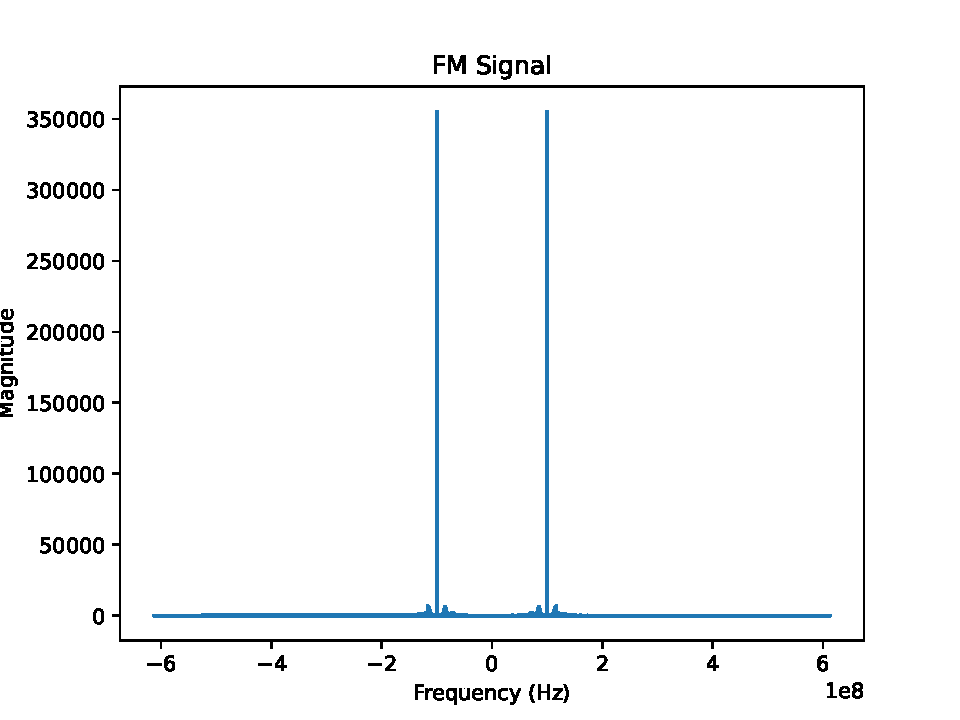
\includegraphics[width=\columnwidth]{fm/tx/figs/tx_spec.pdf} 
\caption{Plot of spectrum of transmitted signal.}
\label{fig:Trans}
\end{figure}
\item Compute and plot the PSD of the message signal using 
\eqref{eq:app-psd-def}.
\\
	\solution
Executing	
\begin{lstlisting}
python3 fm/tx/codes/tx_psd.py
\end{lstlisting}

\begin{figure}[H]
\centering
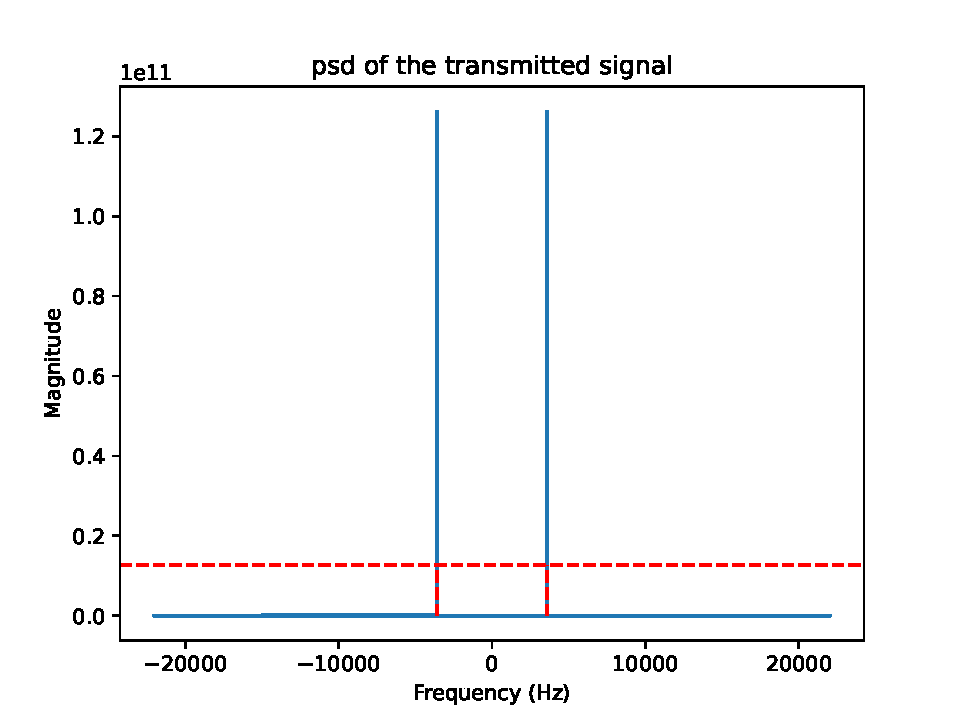
\includegraphics[width=\columnwidth]{fm/tx/figs/tx_psd.pdf}
\caption{Plot of PSD of the message signal.}
\label{fig:fm_PSD}
\end{figure}
\item Compute the bandwidth of the transmitted signal.
\\
\solution
Executing
\begin{lstlisting}
python3 fm/tx/codes/tx_bw.py
\end{lstlisting}
gives the bandwidth of the transmitted signal as 7190.69574 Hz
\\
The threshold of the transmitted signal from the plot is 1.2621 $\times 10^{10}$
\\
The maximum and minimum frequencies are 3595.34787 Hz and -3595.34787 respectively.
\\
Therefore bandwidth is\\
\begin{align}
\centering
f_{max}-f_{min} = 3595.34787-(-3595.34787) = 7190.69574 Hz
\end{align}
\iffalse
\begin{lstlisting}
/fm/FM/codes/mod.py
\end{lstlisting}
\fi
\end{enumerate}
